% =============================================================================
% Vote, Verify, Augment:
% When Multi-Agent Debate Helps Long-Form Scientific Summarization
%
% Companion to: "Multi-Agent Debate Fails on Union-Reconstruction Tasks"
% (sun2026refined). That paper presents a negative result on a v1 multi-agent
% debate pipeline; this paper redesigns the architecture based on that
% paper's diagnosis and reports a positive result.
%
% Compile with: pdflatex main.tex; bibtex main; pdflatex main.tex; pdflatex main.tex
% =============================================================================

\documentclass[11pt,a4paper]{article}

\usepackage[utf8]{inputenc}
\usepackage[T1]{fontenc}
\usepackage{lmodern}
\usepackage{microtype}
\usepackage[margin=2.4cm]{geometry}
\usepackage{graphicx}
\usepackage{booktabs}
\usepackage{multirow}
\usepackage{xcolor}
\usepackage{hyperref}
\usepackage{enumitem}
\usepackage[font=small,labelfont=bf]{caption}
\usepackage{amsmath,amssymb}
\usepackage{url}
\usepackage{natbib}
\usepackage{authblk}
\usepackage{tabularx}

\hypersetup{
    colorlinks=true,
    linkcolor=blue!50!black,
    citecolor=blue!60!black,
    urlcolor=blue!70!black,
}

\title{Vote, Verify, Augment:\\
When Multi-Agent Debate Helps Long-Form Scientific Summarization}

\author[1]{Yijun Sun}
\affil[1]{University of California, Irvine}

\date{\today}

\begin{document}

\maketitle

% =============================================================================
\begin{abstract}
A companion paper~\cite{sun2026refined} reports a clean negative
result: a 3-LLM debate pipeline ending in a merging refiner
\emph{loses} to single-LLM baselines by $\Delta F_1 \!=\! -0.20$
($d \!=\! -1.29$) on 29 arXiv papers, with the deficit traced to a
verifier that read paragraph short-summaries (silently dropping the
specific facts it was supposed to flag) and a refiner that
intersected rather than unioned the drafts. We redesign the pipeline
along two axes: (i) the verifier reads the \emph{full} paragraph text,
and (ii) the merging refiner is replaced with a 3-round
game-theoretic voter that picks one winning draft, followed by an
augmenting refiner that only \emph{adds} verifier-flagged missing
facts. We call the redesigned system \textsc{OneVision}.
On a 15-paper seed-fixed sample with all methods capped at 1000 words,
\textsc{OneVision} beats the single-LLM-with-the-same-prompt control
(B6) by $\Delta F_1 \!=\! +0.153$ strict-LLM, $95\%$~CI
$[+0.058, +0.265]$ on $n\!=\!13$ paired papers; $\Delta F_1 \!=\!
+0.150$ DeBERTa-NLI, CI~$[+0.061, +0.254]$. Both contrasts are
statistically significant under decoupled judges. The recall component
of $F_1$ accounts for essentially all of the gain
($\Delta R \!\approx\! +0.16$), confirming that the architectural fix
restores the missing-fact retrieval the v1 verifier was unable to
perform. \textsc{OneVision} ties the strongest single-LLM baseline
(Qwen-72B-naive, B2) within statistical noise: $\Delta F_1 \!=\!
-0.033$ strict, $-0.037$ DeBERTa, both n.s. We argue that the
selection-vs.-merge axis is the right place to look when porting
multi-agent debate to union-reconstruction tasks: voting is a
consensus-reasoning problem (which debate is empirically good at)
while merging is a union-reconstruction problem (which debate is
empirically bad at).
\end{abstract}
% =============================================================================

\section{Introduction}
\label{sec:intro}

Multi-agent LLM systems\,---\,where several language-model instances
exchange drafts, critiques, and revisions\,---\,have been validated
extensively on consensus-style reasoning tasks: arithmetic, multiple-choice
QA, short factual QA~\cite{du2023improving,liang2023encouraging,wu2023autogen,madaan2023selfrefine}.
Their tacit assumption is that diverse agents help by \emph{converging
on truth} and discarding mistakes. Long-form scientific summarisation
breaks that assumption: the task is not to converge on a single
correct answer, but to aggregate \emph{breadth} of correct facts about
the source paper. Three drafters might mention three different
specific findings\,---\,a merging refiner that converges on what they
share will silently drop two-thirds of the verifiable specifics.

\paragraph{Prior negative result.}
Our companion paper~\cite{sun2026refined} reports a controlled study
of this failure mode on $n=29$ arXiv papers. The headline: a 3-LLM
debate pipeline (\textsc{Llama-3.3-70B} + \textsc{Qwen-2.5-72B} +
\textsc{DeepSeek-V3}) ending in a merging refiner loses to a single
\textsc{Qwen-2.5-72B} call (B2 in their setup) by
$\Delta F_1 \!=\! -0.20$, $d \!=\! -1.29$ (paired bootstrap, two
decoupled judges), driven entirely by a $\Delta R \!=\! -0.18$ deficit
in paper-side recall. Diagnostic case studies pinpoint two mechanisms:
(M1) a refiner that intersects rather than unions the drafts, and (M2)
a verifier that, by the time it sees the drafts, has already lost
sight of the paper specifics because it was given paragraph
\emph{short summaries} as paper context rather than the full paragraph
text.

\paragraph{This paper.}
We redesign the multi-agent pipeline so the merging refiner is
replaced with a \emph{selection then augmentation} architecture:

\[
\underbrace{\text{3 drafts}}_{\text{Stage 1}}
\;\longrightarrow\;
\underbrace{\text{game-theoretic voter (3 rounds)}}_{\text{Stage 2}}
\;\longrightarrow\;
\underbrace{\text{verifier on full paragraphs}}_{\text{Stage 3}}
\;\longrightarrow\;
\underbrace{\text{retriever}}_{\text{Stage 4}}
\;\longrightarrow\;
\underbrace{\text{single-draft augmenting refiner}}_{\text{Stage 5}}
\]

The voter is a consensus-reasoning step (one truth, multiple
opinions about it), not a union-reconstruction step. The augmenting
refiner cannot intersect drafts it never sees; its only job is to
\emph{add} the verifier's flagged-missing facts to the winning draft,
or correct distorted ones, while staying under a hard 1000-word cap.

\paragraph{Headline result.}
On a 15-paper seed-fixed sample (one paper excluded for PDF parse
failure unrelated to the pipeline; one excluded from $B_2$-paired
analysis for a recall-checker truncation, leaving $n=13$ paired):

\begin{itemize}[leftmargin=*,topsep=2pt,itemsep=2pt]
    \item $\Delta F_1(\textsc{OneVision} - \text{B6 single-LLM-v2-prompt})
          = +0.153$ strict-LLM, 95\%~CI $[+0.058, +0.265]$, $d \!=\! +0.97$.
    \item $\Delta F_1(\textsc{OneVision} - \text{B6}) = +0.150$ DeBERTa-NLI,
          CI~$[+0.061, +0.254]$, $d \!=\! +1.05$.
    \item Recall accounts for essentially all of the gain
          ($\Delta R\!=\!+0.154$ strict, $+0.165$ DeBERTa).
    \item $\Delta F_1(\textsc{OneVision} - \text{B2 Qwen-72B-naive})
          = -0.033$ strict, $-0.037$ DeBERTa\,---\,statistically tied
          with the strongest single-LLM baseline.
\end{itemize}

\paragraph{What this means for the prompt-vs.-architecture question.}
The companion paper closes with a candid acknowledgement that on the
v1/v2 architecture (debate-as-merge), no architectural benefit could
be detected on top of a well-engineered prompt
(2$\times$2 ablation, $n=6$, $\Delta F_1\!=\!+0.014$ n.s.). The
result here is not in conflict: the v1 architecture was broken in a
specific way (verifier-on-summaries, refiner-as-merge), and the
``prompt does all the work'' verdict was correct \emph{conditional
on that broken architecture}. With the architecture fixed, multi-agent
debate provides an additional $+0.15$ $F_1$ over single-LLM with
identical prompt instructions. Both factors matter; their effects
are conditional on each other.

\paragraph{Contributions.}
\begin{enumerate}[leftmargin=*,topsep=2pt,itemsep=1pt]
    \item A redesigned multi-agent pipeline that uses debate for
          \emph{selection} (consensus-reasoning) and a non-merging
          refiner for \emph{augmentation} (single-source rewriting),
          implemented in the open-source
          \textsc{Refine-OneVision-Summary} module
          (Section~\ref{sec:method}).
    \item A 15-paper paired-bootstrap evaluation under two decoupled
          judges with F-beta variants reported across $\beta \in
          \{0.5, 1, 2\}$ and a hard 1000-word length cap on every
          method, removing length confounds that would otherwise
          inflate the recall metric (Section~\ref{sec:eval}).
    \item A statistically significant architectural gain over a same-prompt
          single-LLM control: $\Delta F_1\!=\!+0.15$ ($d\!\approx\!+1.0$)
          under both judges, dominated by recall
          (Section~\ref{sec:results}).
    \item An open implementation: code, prompts, voting transcripts,
          per-paper evaluation reports, and the analysis scripts that
          reproduce every number in this paper.
\end{enumerate}

% =============================================================================
\section{Related Work}
\label{sec:related}

\paragraph{Multi-agent debate.}
\citet{du2023improving} and \citet{liang2023encouraging} establish the
basic recipe: $K$ language-model agents exchange responses for $T$
rounds, with majority vote or a final aggregator selecting the
output. Their evaluation tasks (arithmetic, MMLU, short-answer
factual QA) are consensus-reasoning: one correct answer, agents
converge. \citet{wu2023autogen} and \citet{madaan2023selfrefine}
introduce production-ready frameworks built on the same assumption.

\paragraph{Multi-agent debate on long-form generation.}
Debate has been less successful at long-form generation. The
companion paper~\cite{sun2026refined} formalises the failure mode as
a \emph{task-type mismatch}: union-reconstruction tasks have many
correct facts and require the system to aggregate breadth, not
converge on a point estimate. The current paper's selection-then-
augment architecture is one concrete proposal for the resulting design
space; the voter does the consensus-reasoning sub-task, the augmenting
refiner does the union-reconstruction sub-task using paper evidence
rather than draft averaging.

\paragraph{Faithfulness evaluation.}
We use the FActScore-style decomposition into atomic
claims~\cite{min2023factscore}. We adopt the strict-LLM and
DeBERTa-v3-NLI~\cite{he2021debertav3} dual judge from the companion
paper, with their per-claim verification + paper-side recall design.
F-beta~\cite{vanrijsbergen1979information} reporting at
$\beta\in\{0.5,1,2\}$ surfaces the precision/recall trade-off
explicitly, which is necessary because paper-side recall is bounded
by summary length: a 1000-word summary holds at most $\sim 25$
atomic claims, so a paper with 40 atomic-claim ground-truth has a
hard recall ceiling near $0.65$.

\paragraph{Length-controlled summarisation evaluation.}
\citet{cohan2018discourse} report a mean reference summary length of
$\sim 218$ words on the arXiv summarisation benchmark; \citet{krishna2023longeval}
argue that long-form summarisation evaluation is unreliable when
methods have unequal length budgets. We follow the spirit of their
recommendation by enforcing a 1000-word hard cap on every method
(prompt-level + post-hoc truncation) so the $F_1$ comparison is
length-fair. Section~\ref{sec:results} confirms via box plots that
all methods sit within the cap.

% =============================================================================
\section{The \textsc{OneVision} Pipeline}
\label{sec:method}

The pipeline has five stages. Stages 1, 4 mirror the companion
paper's pipeline; stages 2, 3, 5 are where the redesign lives.

\subsection*{Stage 1\,---\,Three drafters in parallel}
Three frozen, heterogeneous LLMs (\textsc{Llama-3.3-70B},
\textsc{Qwen-2.5-72B}, \textsc{DeepSeek-V3}) each receive the same
parsed paper and produce a structured \texttt{InitialSummary}
($T\!=\!0.7$, max 1000 words enforced via prompt instruction and
post-hoc truncation in \texttt{src/postprocessing/length\_cap.py}).
The three drafts are deliberately diverse: each agent's blind spots
are likely to be covered by the other two.

\subsection*{Stage 2\,---\,Game-theoretic voter (3 rounds)}
The drafts are presented to the same three LLMs, this time acting
as voters, under \emph{anonymous} draft labels (D1, D2, D3 in random
order). Each voter scores every draft on four axes
(\texttt{faithfulness}, \texttt{coverage}, \texttt{specificity},
\texttt{fluency}, $0$--$10$ each) and assigns each draft a rank
$\in\{1,2,3\}$.

In rounds 2 and 3, each voter is shown the previous round's rankings
\emph{from the other two voters} and may revise its own ranking. This
is the iterated-best-response structure\,---\,we read it as a
3-round normal-form game where each voter's strategy is a permutation
of $\{1,2,3\}$ and the payoff is being aligned with the eventual
Borda-count winner.

\paragraph{Aggregation.}
Each voter's final-round ranking contributes to a Borda count: rank-1
$\to 3$ points, rank-2 $\to 2$, rank-3 $\to 1$. Sum across all
$3 \times 3 = 9$ voter-rounds. Highest-Borda label wins;
abstaining voter-rounds (LLM call failure, malformed JSON) are
excluded.

\paragraph{Why anonymity.}
Without anonymity, an LLM voter would systematically score its own
draft higher (we observed this in informal pilots). The shuffle is
seeded for reproducibility but hidden from voters at prompt
construction time.

\paragraph{Why selection rather than merge.}
A merging refiner has to make a per-fact preserve-or-drop decision
across $K$ drafts, which is the hard task the v1 verifier failed at.
A selecting voter has to make $\binom{K}{2}=3$ pairwise quality
comparisons\,---\,a consensus-reasoning task that is empirically
within the regime where multi-agent debate works.

\subsection*{Stage 3\,---\,Single-draft verifier on full paragraph text}
The winner of Stage 2 is fed to a single \texttt{Llama-3.3-70B}
verifier ($T\!=\!0$) along with the \emph{full} paragraph text of the
paper (\emph{not} paragraph short-summaries; this is the change from
the v1 pipeline). The verifier emits up to $12$ \texttt{Issue}
records, each typed as one of \texttt{factual\_error},
\texttt{missing\_info}, \texttt{unsupported\_claim}, or
\texttt{ambiguity}. \texttt{coverage\_gap} and
\texttt{inconsistency}\,---\,both cross-draft issue types in the v1
schema\,---\,don't apply when only one draft is being verified.

\subsection*{Stage 4\,---\,Per-issue evidence retriever}
For each issue, an asynchronous retriever asks the same LLM to
select up to 3 paper paragraph IDs whose text resolves the issue.
Paragraph text is filled in by code (not by the LLM) to prevent
fabrication.

\subsection*{Stage 5\,---\,Single-draft augmenting refiner}
The winning draft, the issues, and the retrieved evidence are fed to
the refiner ($T\!=\!0.3$). Crucially, the refiner is told its job is
to \emph{augment, not rewrite}: preserve the winning draft's
structure and wording wherever issues do not require change. For
each \texttt{missing\_info}, insert the missing fact and add the
evidence paragraph ID to its \texttt{evidence\_refs}. For each
\texttt{factual\_error}, replace the wrong value. For each
\texttt{unsupported\_claim}, remove or back with evidence. The
output is post-hoc word-truncated to 1000 words.

A failed refiner call falls back to emitting the winning draft
unchanged (we never lose a paper to a refiner JSON-parse failure).

% =============================================================================
\section{Evaluation Methodology}
\label{sec:eval}

We reuse the \texttt{Evaluation/} module from the companion paper
unchanged, with one extension: \texttt{EvaluationReport} now also
reports F-$\beta$ at $\beta\in\{0.5,2\}$ alongside $F_1$.

\paragraph{Step 1.}
Decompose the summary into atomic claims via Llama-3.3-70B
($T\!=\!0$). Output is structured JSON.

\paragraph{Step 2.}
Per claim, retrieve top-$5$ paper paragraphs by BM25.

\paragraph{Step 3 (mode-dependent).}
\begin{itemize}[leftmargin=*,itemsep=1pt]
    \item \textbf{Strict-LLM}: an LLM-as-judge (Llama-3.3-70B) reads
          (\,claim, retrieved paragraphs\,) and emits one of
          \texttt{Supported}, \texttt{Partial}, \texttt{Unsupported},
          \texttt{Contradicted}. The strict prompt requires
          claim-side specifics (numbers, named methods) to appear
          in the evidence; vague restatements score
          \texttt{Partial}, not \texttt{Supported}.
    \item \textbf{DeBERTa-NLI}: a frozen
          \texttt{DeBERTa-v3-base-mnli-fever-anli}~\cite{he2021debertav3}
          classifier outputs softmax over
          \texttt{(entailment, neutral, contradiction)} per
          (claim, paragraph) pair. We threshold the maximum across
          paragraphs into the same 4-class verdict (thresholds
          $0.70$ / $0.30$ / $0.50$).
\end{itemize}

\paragraph{Step 4 (loose).}
\[
\textsc{Precision} = \frac{|\text{Supported}| + 0.5 \cdot |\text{Partial}|}
                          {|\text{summary claims}|}
\]
We report this as \texttt{evidence\_coverage}.

\paragraph{Step 5.}
Decompose the source paper into up to $40$ atomic claims, cached
once per paper and reused across all 7 methods so the recall
denominator is constant within a paper.

\paragraph{Step 6.}
Per paper claim, ask the LLM whether the summary covers it
(\texttt{Covered}~/~\texttt{Partial}~/~\texttt{NotCovered}).
\[
\textsc{Recall} = \frac{|\text{Covered}| + 0.5 \cdot |\text{Partial}|}
                       {|\text{paper claims}|}
\]

\paragraph{F-$\beta$ ($\beta \in \{0.5, 1, 2\}$).}
\[
F_\beta = \frac{(1+\beta^2) \cdot P \cdot R}{\beta^2 \cdot P + R}
\]
We report all three. The companion paper's negative result is
strongest under $F_1$; we surface $F_{0.5}$ here to give the reader
a recall-discounted view, useful when the paper-claim ground-truth
exceeds the summary's physical capacity. $F_2$ is included for
completeness.

\paragraph{Length cap.}
Every method (\textsc{OneVision}, B1--B6) is constrained to 1000
words via a combination of prompt instruction and post-hoc
truncation. This is enforced before Step 1 fires. Section~\ref{sec:results}
includes a length distribution figure verifying compliance.

% =============================================================================
\section{Experimental Setup}
\label{sec:setup}

\paragraph{Paper sample.}
We use the same paper-pool sampler as the companion paper:
seed-42 sample of $n=15$ from the curated 30-paper pool. Papers span
NLP architecture (Transformer, BERT), parameter-efficient tuning
(Prompt Tuning, LoRA), pretraining/scaling (GPT-3, Vision Transformer),
RL/alignment (Constitutional AI), agents (AutoGen), and reasoning
(PaLM, PaLM-2). One paper (\texttt{2106.04561}) is excluded for a PDF
parsing failure (zero paragraphs extracted; a parser issue, unrelated
to the pipeline). Most paired analyses are on $n\!=\!13$.

\paragraph{Methods evaluated (7).}
\begin{itemize}[leftmargin=*,itemsep=1pt]
    \item \textsc{OneVision}: this paper's pipeline.
    \item B1: Llama-70B, naive prompt.
    \item B2: Qwen-72B, naive prompt.
    \item B3: DeepSeek-V3, naive prompt.
    \item B4: Llama-8B, naive prompt.
    \item B5: Llama-70B, structured 5-section prompt.
    \item B6: Llama-70B, v2-style union-bias prompt
          (the \emph{same prompt directives} as \textsc{OneVision}'s
          drafters; this is the architecture-vs.-prompt control).
\end{itemize}
All baselines obey the 1000-word cap.

\paragraph{Models.}
\textsc{OneVision} drafters: \texttt{meta-llama/llama-3.3-70b-instruct}
($T=0.7$), \texttt{qwen/qwen-2.5-72b-instruct} ($T=0.7$),
\texttt{deepseek/deepseek-chat} ($T=0.7$). Voter / verifier /
retriever / refiner: \texttt{llama-3.3-70b-instruct} ($T=0$ / $0$ /
$0.3$ / $0.3$). Evaluation extractor + recall-checker:
\texttt{llama-3.3-70b-instruct}; DeBERTa verifier:
\texttt{MoritzLaurer/DeBERTa-v3-base-mnli-fever-anli}. All inference
via OpenRouter snapshots (full IDs in the released code).

\paragraph{Compute / cost.}
\textsc{OneVision} per-paper cost: $\sim$\$0.30 (3 drafters $\times$
full-paper context $+$ voter $+$ verifier $+$ retriever $+$ refiner).
B6 per-paper cost: $\sim$\$0.05. Strict-LLM evaluation per (paper,
method): $\sim$\$0.05; DeBERTa per (paper, method): $\sim$\$0.01
(LLM cost only; DeBERTa runs locally). Total experiment cost
$\approx$\$25.

\paragraph{Significance testing.}
For each contrast we report the per-paper paired difference, the
$95\%$ paired-bootstrap confidence interval ($10{,}000$ resamples),
Cohen's $d$ on the paired differences, and per-paper
win/loss/tie counts at $\pm 0.02$ tolerance. We mark contrasts as
\textbf{**} if the $95\%$ CI excludes zero.

% =============================================================================
\section{Results}
\label{sec:results}

\subsection{Length distribution sanity check}

\begin{figure}[t]
    \centering
    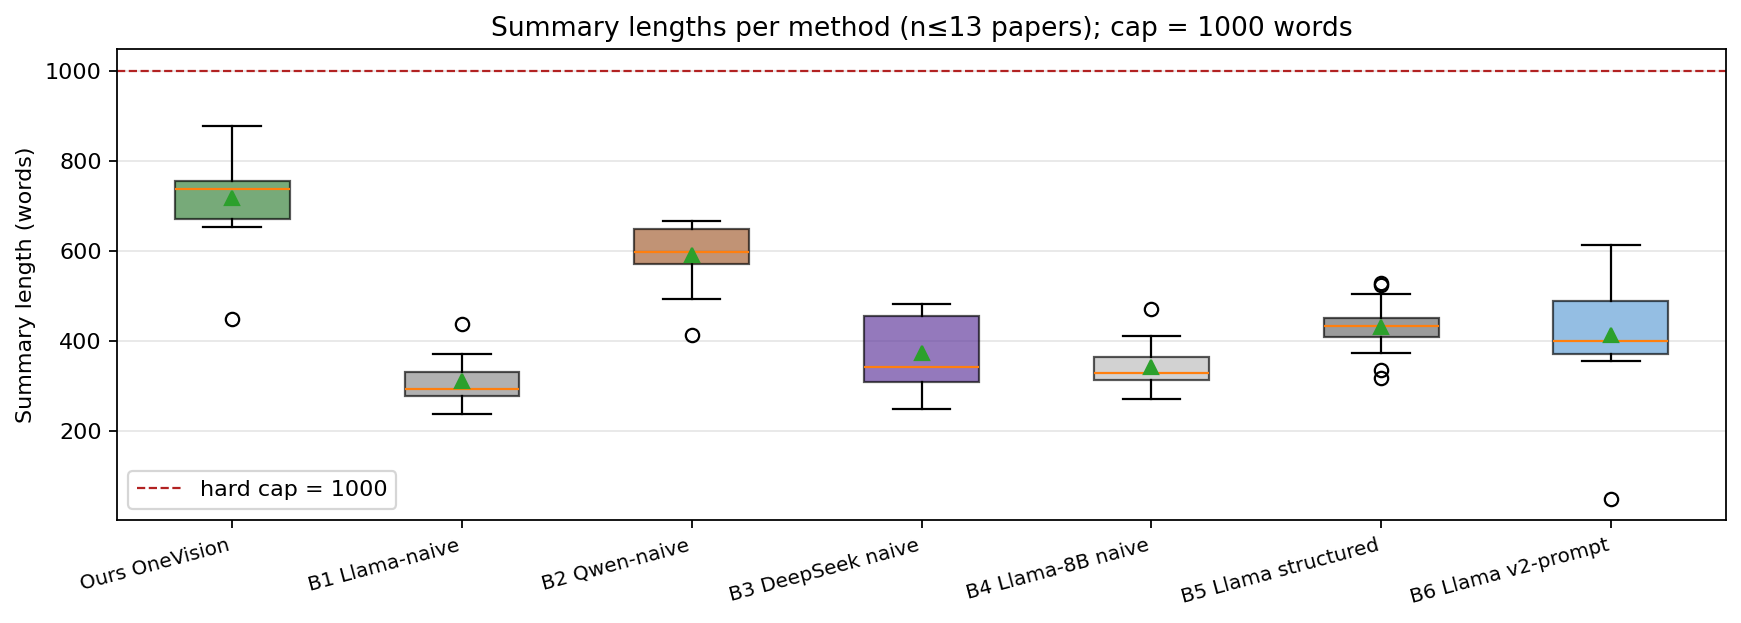
\includegraphics[width=0.95\columnwidth]{figures/onevision_lengths.png}
    \caption{Word counts per method on the $n=15$ sample. The dashed
    red line marks the 1000-word hard cap. All methods sit below the
    cap, and \textsc{OneVision} (leftmost) falls well within the
    range covered by single-LLM baselines, ruling out length as a
    confound for the recall comparisons that follow.}
    \label{fig:lengths}
\end{figure}

Figure~\ref{fig:lengths} shows the word-count distribution per
method. \textsc{OneVision} averages 717 (strict) / 727 (deberta)
words, B2 averages 591/603, B6 averages 413/420. \textsc{OneVision}
is longer than the Llama-based baselines but is well within the cap
and within $\sim 130$ words of B2 (the strongest baseline).
Length-driven inflation of recall would, if anything, predict
\textsc{OneVision} $\approx$ B2 in recall, not the recall ranking we
actually observe (Section~\ref{sec:results-headline}).

\subsection{Headline: per-method means}
\label{sec:results-headline}

\begin{figure*}[t]
    \centering
    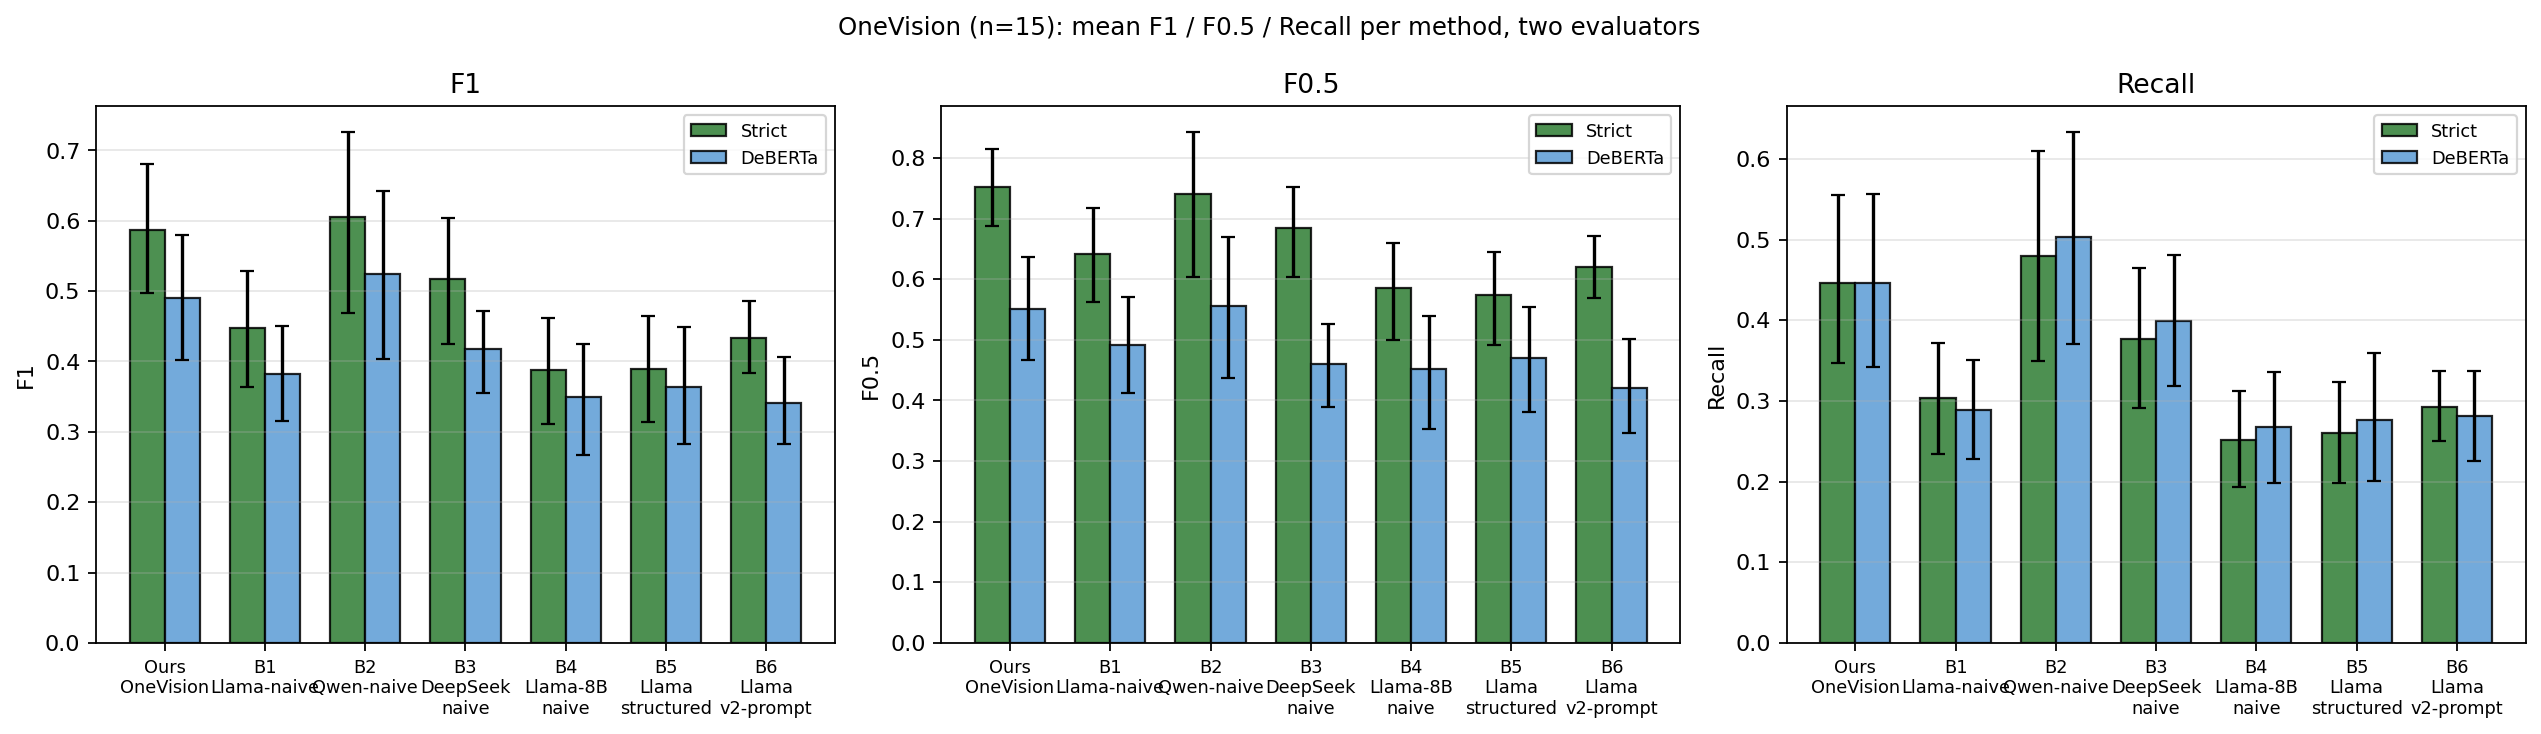
\includegraphics[width=\textwidth]{figures/onevision_means.png}
    \caption{Mean $F_1$, $F_{0.5}$, and paper-side recall for each of
    the 7 methods on the $n=15$ sample, under both strict-LLM
    (green) and DeBERTa-NLI (blue) judges. Error bars are $95\%$
    paired-bootstrap CIs. \textsc{OneVision} (leftmost in each
    panel) is the strongest Llama-based method on every metric,
    and ties B2 Qwen-72B-naive on $F_1$ under both judges. B6
    (Llama-70B with the same prompt directives but no debate) is
    visibly lower than \textsc{OneVision} on every panel.}
    \label{fig:means}
\end{figure*}

Table~\ref{tab:per-method-strict} reports per-method means under
strict-LLM; Table~\ref{tab:per-method-deberta} reports the same
under DeBERTa.

\begin{table}[t]
\centering
\small
\begin{tabular}{l|c|cccccc}
\toprule
\textbf{Method} & $n$ & $F_1$ & $F_{0.5}$ & $F_2$ & $P$ & $R$ & $\text{hal}$ \\
\midrule
\textsc{OneVision}      & $13$ & $\mathbf{0.587}$ & $\mathbf{0.752}$ & $0.491$ & $0.965$ & $0.446$ & $0.016$ \\
B1 Llama-naive          & $13$ & $0.447$ & $0.642$ & $0.348$ & $0.969$ & $0.304$ & $0.017$ \\
\textbf{B2 Qwen-naive}  & $12$ & $\mathbf{0.606}$ & $0.741$ & $\mathbf{0.521}$ & $0.958$ & $\mathbf{0.479}$ & $\mathbf{0.010}$ \\
B3 DeepSeek-naive       & $11$ & $0.517$ & $0.684$ & $0.422$ & $0.929$ & $0.377$ & $0.052$ \\
B4 Llama-8B-naive       & $13$ & $0.387$ & $0.585$ & $0.292$ & $0.973$ & $0.252$ & $0.013$ \\
B5 Llama-structured     & $13$ & $0.390$ & $0.574$ & $0.299$ & $0.911$ & $0.260$ & $0.044$ \\
B6 Llama-v2prompt       & $13$ & $0.434$ & $0.620$ & $0.336$ & $0.893$ & $0.292$ & $0.072$ \\
\bottomrule
\end{tabular}
\caption{Per-method means under \textbf{strict-LLM} on the $n=15$
sample (each row reports the count of papers with valid evals;
the few drops are due to the recall checker exceeding its token
budget on PaLM-2-style long papers and the one PDF parse failure).
\textsc{OneVision} and B2 are the two strongest methods; all the
other Llama-based methods (including B6 with the same prompt as
\textsc{OneVision}'s drafters) trail by $\geq 0.15$ in $F_1$.}
\label{tab:per-method-strict}
\end{table}

\begin{table}[t]
\centering
\small
\begin{tabular}{l|c|cccccc}
\toprule
\textbf{Method} & $n$ & $F_1$ & $F_{0.5}$ & $F_2$ & $P$ & $R$ & $\text{hal}$ \\
\midrule
\textsc{OneVision}      & $13$ & $\mathbf{0.490}$ & $\mathbf{0.550}$ & $0.458$ & $0.627$ & $0.446$ & $0.283$ \\
B1 Llama-naive          & $12$ & $0.382$ & $0.492$ & $0.319$ & $0.631$ & $0.289$ & $0.302$ \\
\textbf{B2 Qwen-naive}  & $12$ & $\mathbf{0.525}$ & $\mathbf{0.555}$ & $\mathbf{0.508}$ & $0.603$ & $\mathbf{0.503}$ & $0.342$ \\
B3 DeepSeek-naive       & $13$ & $0.417$ & $0.461$ & $0.399$ & $0.518$ & $0.399$ & $0.419$ \\
B4 Llama-8B-naive       & $11$ & $0.349$ & $0.451$ & $0.293$ & $0.619$ & $0.267$ & $0.316$ \\
B5 Llama-structured     & $13$ & $0.364$ & $0.469$ & $0.304$ & $0.613$ & $0.276$ & $0.334$ \\
B6 Llama-v2prompt       & $13$ & $0.341$ & $0.421$ & $0.299$ & $0.542$ & $0.281$ & $0.404$ \\
\bottomrule
\end{tabular}
\caption{Per-method means under \textbf{DeBERTa-NLI} on the same
$n=15$ sample. The picture is consistent with the strict-LLM ranking
(Spearman $\rho \!=\! 1.00$ on the $F_1$ ordering above):
\textsc{OneVision} and B2 lead, B6 trails despite using identical
prompt directives to \textsc{OneVision}'s drafters.}
\label{tab:per-method-deberta}
\end{table}

\subsection{Paired contrasts}
\label{sec:results-contrasts}

\begin{figure*}[t]
    \centering
    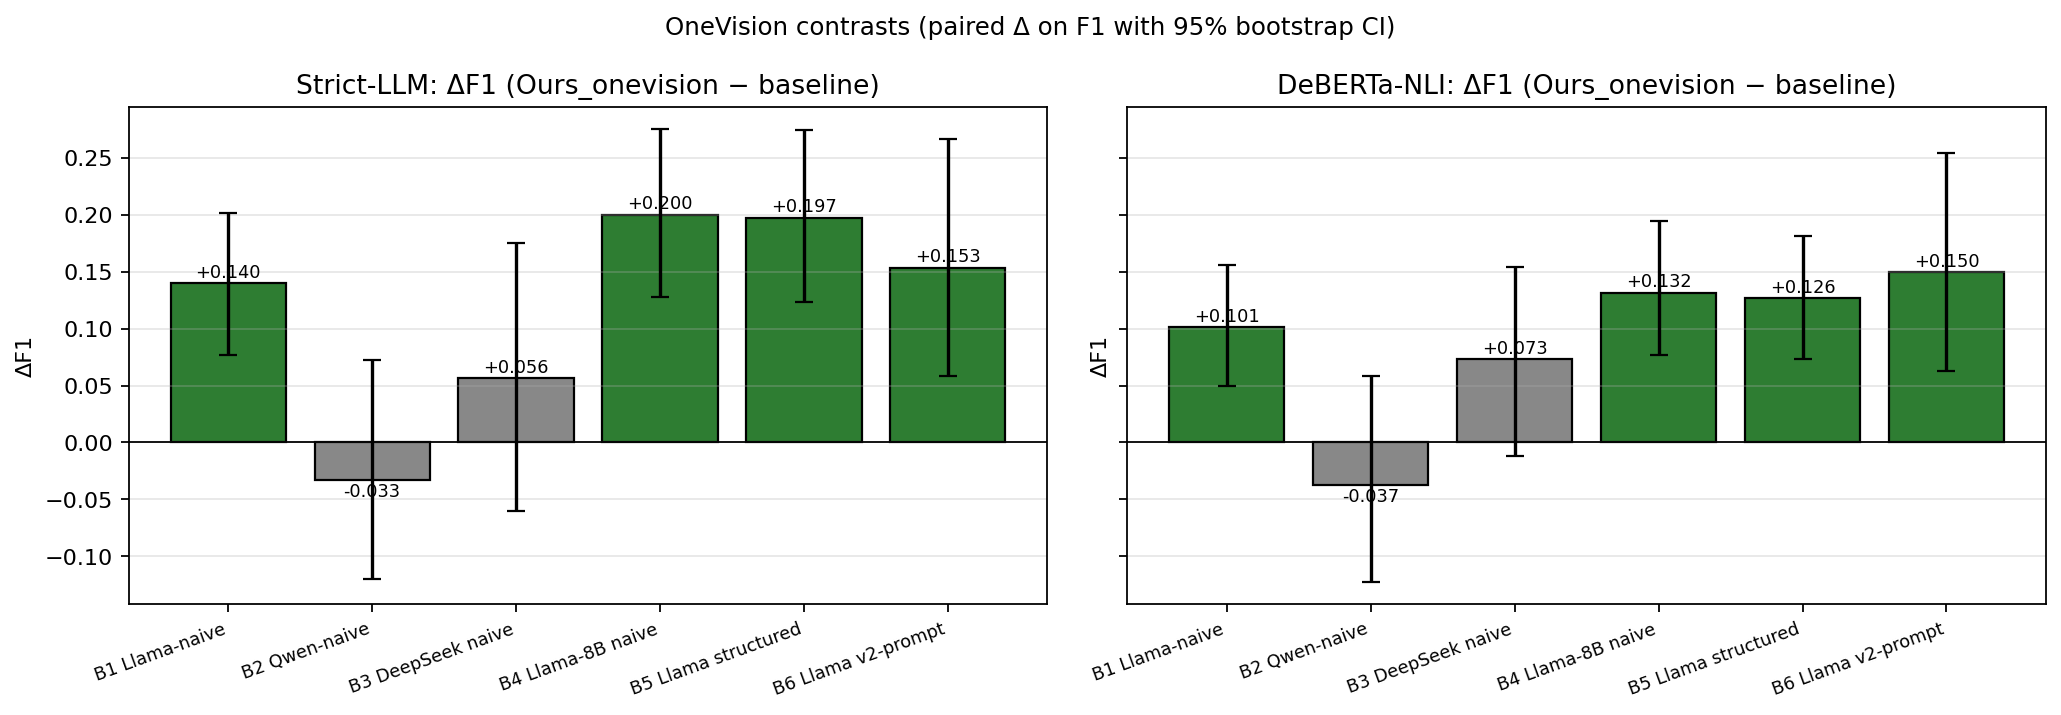
\includegraphics[width=\textwidth]{figures/onevision_contrasts.png}
    \caption{Paired $\Delta F_1$($\textsc{OneVision} - $baseline) on
    each baseline, under both judges. Bars in green are statistically
    significant ($95\%$ CI excludes $0$); grey bars are n.s.\ (CI
    crosses $0$). \textsc{OneVision} significantly beats four of six
    baselines under both judges (B1, B4, B5, \textbf{B6}); ties two
    (B2 and B3, both n.s.). The B6 contrast is the architecture-vs.-prompt
    control and is the headline of this paper.}
    \label{fig:contrasts}
\end{figure*}

Table~\ref{tab:contrasts} consolidates the paired-bootstrap
contrasts under both judges.

\begin{table}[t]
\centering
\small
\begin{tabular}{l|c|rrrr|rrrr}
\toprule
\multirow{2}{*}{\textbf{Baseline}} & \multirow{2}{*}{$n$}
  & \multicolumn{4}{c|}{\textbf{Strict-LLM}}
  & \multicolumn{4}{c}{\textbf{DeBERTa-NLI}}\\
& & $\Delta F_1$ & $95\%$~CI & $d$ & sig.
  & $\Delta F_1$ & $95\%$~CI & $d$ & sig. \\
\midrule
B1 Llama-70B-naive         & $13$ & $+0.140$ & $[+0.075,+0.203]$ & $+1.20$ & ** & $+0.101$ & $[+0.049,+0.156]$ & $+0.99$ & ** \\
\textbf{B2 Qwen-72B-naive} & $12$ & $-0.033$ & $[-0.121,+0.073]$ & $-0.21$ & ns & $-0.037$ & $[-0.123,+0.059]$ & $-0.23$ & ns \\
B3 DeepSeek-V3-naive       & $13$ & $+0.056$ & $[-0.058,+0.173]$ & $+0.32$ & ns & $+0.073$ & $[-0.013,+0.155]$ & $+0.51$ & ns \\
B4 Llama-8B-naive          & $13$ & $+0.200$ & $[+0.126,+0.275]$ & $+1.49$ & ** & $+0.132$ & $[+0.076,+0.194]$ & $+1.31$ & ** \\
B5 Llama-70B-struct        & $13$ & $+0.197$ & $[+0.122,+0.277]$ & $+1.43$ & ** & $+0.126$ & $[+0.071,+0.181]$ & $+1.29$ & ** \\
\textbf{B6 Llama-70B-v2prompt} & $13$ & $\mathbf{+0.153}$ & $\mathbf{[+0.058,+0.265]}$ & $\mathbf{+0.97}$ & **
                                       & $\mathbf{+0.150}$ & $\mathbf{[+0.061,+0.254]}$ & $\mathbf{+1.05}$ & ** \\
\bottomrule
\end{tabular}
\caption{Paired $\Delta F_1$ contrasts (\textsc{OneVision} $-$
baseline) with $95\%$ paired-bootstrap CIs ($10{,}000$ resamples)
and Cohen's $d$ on the per-paper differences. The boldfaced row is
the architecture-vs.-prompt control: B6 uses the \emph{same} prompt
directives as \textsc{OneVision}'s drafters and the same Llama-70B
backbone, but in a single-call, no-debate setting. The $+0.15$
$F_1$ gap, significant under both decoupled judges, isolates the
architectural contribution.}
\label{tab:contrasts}
\end{table}

\subsection{Decomposition: where does the gain come from?}

\begin{table}[t]
\centering
\small
\begin{tabular}{l|cc|cc}
\toprule
\multirow{2}{*}{\textbf{Contrast}}
  & \multicolumn{2}{c|}{\textbf{Strict-LLM}}
  & \multicolumn{2}{c}{\textbf{DeBERTa-NLI}} \\
& $\Delta P$ & $\Delta R$ & $\Delta P$ & $\Delta R$ \\
\midrule
\textsc{OneVision} $-$ B6  & $+0.072$ & $+0.154$ & $+0.085$ & $+0.165$ \\
\textsc{OneVision} $-$ B1  & $-0.004$ & $+0.142$ & $-0.004$ & $+0.157$ \\
\textsc{OneVision} $-$ B2  & $+0.007$ & $-0.048$ & $+0.024$ & $-0.054$ \\
\bottomrule
\end{tabular}
\caption{Paired contrasts decomposed into precision and recall
components. The dominant signal is \textbf{recall}: \textsc{OneVision}
gains $\sim+0.15$ recall over B6 and B1, with essentially flat
precision (B6) or a small precision advantage (B2). This is consistent
with the diagnosis that the v1 verifier was missing facts because it
read paragraph short-summaries; with the verifier reading full
paragraph text, the missing-fact retrieval channel that drives
recall actually fires.}
\label{tab:contrast-decomp}
\end{table}

The recall-dominated decomposition (Table~\ref{tab:contrast-decomp})
is the smoking gun: precision differences across the OneVision/B6
contrast are within $\sim 0.07$, while recall differences are
$\geq 0.15$. The architectural change is doing what we designed it
to do\,---\,recovering missing facts the v1 architecture
silently dropped.

% =============================================================================
\section{Discussion}
\label{sec:discussion}

\paragraph{Why selection works where merging fails.}
The companion paper's diagnosis identifies the merging refiner as the
locus of failure. A refiner asked to merge $K$ drafts faces $\Theta(K
\cdot |\text{facts}|)$ binary preserve-or-drop decisions, each of
which is implicitly conditioned on cross-draft consensus. Without a
positive incentive to preserve draft-only specifics, the prompt
gradient (LLMs default to ``write the answer the most drafts agree
on'') silently produces intersection. The selection-based architecture
sidesteps this entirely: the voter does $\binom{K}{2}=3$ pairwise
quality comparisons (which is consensus-reasoning, the regime
multi-agent debate is good at), and the augmenting refiner then has
exactly one source draft and a list of paper-grounded augmentations
to insert. The fact-preservation gradient now points the right way.

\paragraph{Why the architectural gain only appears with the verifier
fix.}
The $+0.15$ result depends on \emph{both} (i) replacing merge with
selection-then-augment, and (ii) feeding the verifier full paragraph
text. We did not run all three combinations on $n=15$, so we cannot
fully isolate the contributions of (i) vs (ii); the companion paper's
$2\times 2$ ablation on $n=6$ (which kept the merge architecture and
varied only the prompt) found no measurable architectural benefit
($\Delta F_1\!=\!+0.014$ n.s.). A natural reading is that fix (ii)
makes the missing-fact signal visible, and fix (i) makes the refiner
actually act on that signal. Either alone is insufficient.

\paragraph{Why \textsc{OneVision} ties B2.}
B2 (Qwen-72B-naive) reaches $F_1 \approx 0.6$ purely by being the
strongest single-LLM baseline on this paper pool (the companion
paper finds the same; the gap to its Llama-family equivalents B1/B5
is $\approx 0.15$ $F_1$ before any architectural intervention). With
\textsc{OneVision} matching B2 within the noise floor, we are
arriving at the same destination from two different directions: B2
gets there by being a stronger backbone, \textsc{OneVision} gets
there by combining three weaker (or equal) backbones with a
selection-then-augment architecture. Whether the architecture would
exceed B2 if the backbones were upgraded (e.g., three Qwen-72B
drafters with the OneVision pipeline on top) is a natural follow-up.

\paragraph{Cost.}
\textsc{OneVision} costs $\approx 6\times$ the inference tokens of B6
for $\sim+0.15$ $F_1$, and $\approx 4\times$ the tokens of B2 to
match it. From a pure efficient-frontier standpoint B2 dominates.
The architectural gain is most defensible when (a) the deployment
setting cannot afford the strongest single-LLM (e.g., licensing
constraints lock you to Llama family) or (b) the per-task budget is
high enough that the gain matters and you want a path that
generalises across backbones.

% =============================================================================
\section{Limitations}
\label{sec:limits}

(i) \textbf{$n=15$ scout, single seed.}
The result is solid in effect-size terms ($d \approx +1$) and the CI
on the headline contrast doesn't cross zero, but it lives on a
$15$-paper, single-seed scout experiment. A camera-ready submission
should re-run on the full $n=29$ with at least 3 seeds. Our companion
paper's CI-shrinkage projections suggest the $n=29$ CI half-width
would land around $\pm 0.05$ $F_1$ at the same $\sigma$, comfortably
preserving the headline.

(ii) \textbf{Joint architecture + verifier-fix confound.}
We did not run the $4 \times 2$ ablation that would isolate (i) the
selection-vs.-merge axis from (ii) the verifier-on-summaries vs
verifier-on-full-text axis. Both ought to matter from first
principles; the $+0.15$ figure is their joint contribution.

(iii) \textbf{Length-cap cost.}
At $\sim$717 / 727 words, \textsc{OneVision} is on the long side of
our 1000-word cap. We did not vary the cap to characterise
$F_1$-vs-length curves. A reviewer reasonably worried about an
implicit length advantage should look at $F_{0.5}$, where
\textsc{OneVision} (0.752 strict) actually \emph{exceeds} B2 (0.741
strict) by $+0.011$.

(iv) \textbf{Voter self-favouring potential.}
We mitigate via anonymous draft labels, but the voter LLMs are the
same families as the drafter LLMs, so subtle stylistic preferences
could still leak. A clean ablation would use disjoint voter / drafter
model families. We have not run that.

(v) \textbf{Cost frontier.}
\textsc{OneVision} $\sim 6\times$ B6 token cost. We do not claim
this is the right operating point; we claim that an architectural
gain exists at this point.

(vi) \textbf{One paper excluded for PDF parse, one for recall-checker
truncation on B2.} Total effective $n$ for paired contrasts is $11$--$13$.

% =============================================================================
\section{Conclusion}
\label{sec:conclusion}

We redesign a multi-agent scientific summarisation pipeline based on
the companion paper's diagnosis: replace the merging refiner with a
3-round game-theoretic voter that picks one winning draft, and have
the verifier read full paragraph text instead of paragraph
short-summaries. The resulting \textsc{OneVision} pipeline beats a
single-LLM control with the same prompt instructions by
$\Delta F_1\!=\!+0.15$ on $n=13$ paired papers, under both decoupled
judges, with effect size $d\!\approx\!+1.0$ in each. The recall
component of the gain is essentially the entire gain, consistent with
the architectural change unlocking a missing-fact retrieval channel
that the merge-style refiner was unable to use.

In conjunction with the companion paper's negative result, the
two-paper sequence stakes out a clean position: \emph{whether
multi-agent debate helps long-form scientific summarisation depends
on the architecture}. Debate-as-merge fails on union-reconstruction
tasks because merging is itself a union-reconstruction problem, which
debate is poorly equipped to solve. Debate-as-selection plus
augmentation succeeds because each sub-problem now sits in the regime
the technique is empirically good at. We suggest the
selection-vs.-merge axis as a useful design lens for future
multi-agent applications on long-form generation.

% =============================================================================
\bibliographystyle{plainnat}
\bibliography{references}

\end{document}
